
Recall that when we write $\vec x=\mat{2\\3}$, what we actually mean is $\vec x=2\xhat+3\yhat$. The numbers $2$
and $3$ are called the coordinates of the vector $\vec x$ with respect to the standard basis.  However, in general,
subspaces have many bases, and so it is possible to represent a single vector in many ways as coordinates with
respect to \emph{many} bases.

Let $\vec x=\mat{2\\3}$; let $\mathcal E=\Set{\xhat,\yhat}$ be the standard basis for $\R^2$ and let
$\mathcal B=\Set{\vec b_1,\vec b_2}$ where $\vec b_1=\mat{1\\1}$ and $\vec b_2=\mat{1\\2}$ be another
basis for $\R^2$. Now, the coordinates of $\vec x$ with respect to $\mathcal E$ are $(2,3)$, but
the coordinates of $\vec x$ with respect to $\mathcal B$ are $(1,1)$.

XXX Figure

The coordinates $(2,3)$ and $(1,1)$ represent $\vec x$ equally well, and when solving problems, we should pick the
coordinates that make our problem the easiest\footnote{ For example, maybe in one choice of coordinates, we can avoid all 
fractions in our calculations---this could be good if you're programming a computer that rounds it.}. However, now that we
are representing vectors in multiple bases, we need a way to keep track of what coordinates correspond to which basis.

\SavedDefinitionRender{RepresentationinaBasis}

\begin{example}
	Let $\mathcal E=\Set{\xhat,\yhat}$ be the standard basis for $\R^2$ and let $\mathcal B=\Set{\vec b_1,\vec b_2}$
	where $\vec b_1=\xhat+\yhat$, and $\vec b_2 =3\yhat$ be another basis for $\R^2$. Given that $\vec v=2\xhat-\yhat$, 
	find $[\vec v]_{\mathcal E}$ and $[\vec v]_{\mathcal B}$.

	Given that $\vec v=2\xhat-\yhat$, we see
	\[
	    [\vec v]_{\mathcal E}=\mat{2\\-1}.
	\]
	To find $[\vec v]_{\mathcal B}$, we can use a system of equations to find $\vec v$ as a linear combination of $\vec b_1$ and $\vec b_2$. 
	
	First, set 
	\[
		\vec v = x\vec b_1 + y\vec b_2    
	\]
	for some unknown scalars $x$ and $y$. Then, since on the one hand,
	\[
	    \vec v = 2\xhat-\yhat
	\]
	and on the other hand, 
	\[
	    \vec v  = x\vec b_1 + y\vec b_2= x(\xhat+\yhat)+3y\yhat=x\xhat+(x+3y)\yhat,
	\]
	equating the two equations above, we have
	\[
	    2\xhat-\yhat = x\xhat+(x+3y)\yhat.
	\]
	Therefore, solving the system 
	\[
	    \sysdelim\{.
		\systeme{
			x=2,
			x+3y=-1
		},
	\]
	we have $\vec v=2\vec b_1 - \vec b_2$. That is,
	\[
	   [\vec v]_{\mathcal B}=\mat{2\\-1}. 
	\]
\end{example}

\Heading{Notation Conventions}
In light of this notation, we need to revisit some past notation. Again, we have been writing $\vec x=\mat{1\\3}$ to mean
$\vec x=2\xhat+3\yhat$. However, given the representation-in-a-basis notation, we should be writing
\[
	\vec x=\mat{2\\3}_{\mathcal E},
\]
where $\mathcal E$ is the standard basis for $\R^2$. We should write $\mat{2\\3}_{\mathcal E}$ because the coordinates $(2,3)$
refer to \emph{different} vectors for \emph{different} bases. However, most of the time we are only thinking about the standard
basis. So, the convention we will follow is:
\begin{itemize}
	\item If a problem involves only one basis, we may write $\mat{x\\y}$ to mean $\mat{x\\y}_{\mathcal E}$ where
	$\mathcal E$ is the standard basis.
	\item If there are multiple bases in a problem, we will always write $\mat{x\\y}_{\mathcal X}$ to specify a vector in
	coordinates relative to a particular basis $\mathcal X$.
\end{itemize}

\begin{emphbox}[Takeaway]
	If a problem only involves the standard basis, we may use the notation we always have. If a problem involves
	multiple bases, we must \emph{always} use representation-in-a-basis notation.
\end{emphbox}


\Heading{True Vectors vs\mbox{.} Representations}

\begin{center}
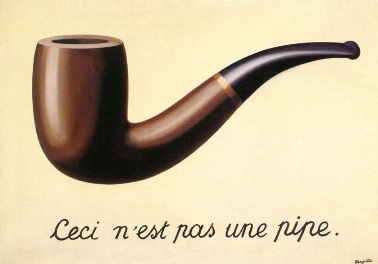
\includegraphics[width=3in]{images/MagrittePipe.jpg}\footnote{Image taken from Wikipedia: \url{https://en.wikipedia.org/wiki/File:MagrittePipe.jpg}} 
\end{center}
The Belgian surrealist Ren\'e Magritte painted the work above, which is subtitled, ``This is not a pipe''. Why? Because, of course, it is not
a pipe. It is a painting of a pipe! In this work, Magritte points out a distinction that will soon become very important to
us---the distinction between an object and a representation of that object.



Let $\vec x=2\xhat+3\yhat\in \R^2$. The vector $\vec x$ is a \emph{real-life geometrical thing}, and to
emphasize this, we will call $\vec x$ a \emph{true} vector. In contrast, when we write
the column matrix $[\vec x]_{\mathcal E}=\mat{2\\3}$, we are writing a \emph{list of numbers}. The list of
numbers $\mat{2\\3}$ has no meaning until we give it a meaning by assigning it a basis. For example,
by writing $\mat{2\\3}_{\mathcal E}$ we declare that the numbers $2$ and $3$ are coefficients of $\xhat$ and
$\yhat$. By writing $\mat{2\\3}_{\mathcal B}$ where $\mathcal B=\Set{\vec b_1,\vec b_2}$,
we declare that the numbers $2$ and $3$ are coefficients of $\vec b_1$ and $\vec b_2$. Since a list of numbers
without a basis has no meaning, we must write
\[
	\vec x\,\,{\color{Red}\neq}\,\,\, [\vec x]_{\mathcal E}=\mat{2\\3},
\]
since the left side of the equation is a \emph{true vector} and the right side is a \emph{list of numbers}. Similarly,
we must write
\[
	[\vec x]_{\mathcal E}\,\,{\color{Red}\neq}\,\,\, \mat{2\\3}_{\mathcal E}=\vec x,
\]
since the left side is a \emph{list of numbers} and the right side is a \emph{true vector}.

To help keep the notation straight in your head, for a basis $\mathcal X$, remember the rule
\[
	[\text{true vector}]_{\mathcal X} = \text{list of numbers}\qquad\text{and}\qquad
	[\text{list of numbers}]_{\mathcal X} =\text{true vector}.
\]

It's easy to get confused when answering questions that involve multiple bases; precision will
make these problems much easier.

\Heading{Orientation of a Basis}
How can you tell the difference between a hand and a foot? They're similar in structure\footnote{ We might
say hands and feet are \emph{topologically} equivalent.}---a hand has five
fingers and a foot has five toes---but they're different in shape---fingers are much longer than toes and the thumb sticks off
the hand at a different angle than the big toe sticks off the foot.

How about a harder question: how can you tell the difference between a left hand and a right hand? Any length
or angle measurement you make on an (idealized) left hand or right hand will be identical. But, we know they're different
because they differ in \emph{orientation}\footnote{ Other words for orientation include \emph{chirality} and \emph{handedness}.}.

We'll build up to the definition of orientation in stages. Consider the ordered bases $\mathcal E$, $\mathcal A$, and
$\mathcal B$ shown below.

\begin{center}
	\begin{tikzpicture}[scale=2]
		\begin{scope}[cm={1,0,0,1,(0,0)}, mypink, thick]
			\begin{scope}[black!30!white]
				\draw[ ->] (0,0) -- (1,0) node [midway, below] {$\xhat$};
				\draw[densely dotted, ->] (0,0) -- (0,1) node [midway, left] {$\yhat$};
			\end{scope}
			\begin{scope}[rotate=60]
				\draw[ ->] (0,0) -- (1,0) node [above right] {$\vec a_1$};
				\draw[densely dotted, ->] (0,0) -- (0,1) node [above left] {$\vec a_2$};
			\end{scope}
		\end{scope}
		\begin{scope}[cm={1,0,0,1,(3,0)}, myorange, thick]
			\begin{scope}[black!30!white]
				\draw[ ->] (0,0) -- (1,0) node [midway, below] {$\xhat$};
				\draw[densely dotted, ->] (0,0) -- (0,1) node [midway, left] {$\yhat$};
				%\draw[ ->] (0,0) -- (1,0);
				%\draw[densely dotted, ->] (0,0) -- (0,1);
			\end{scope}
			\begin{scope}[rotate=-60,cm={-1,0,0,1,(0,0)}]
				\draw[ ->] (0,0) -- (1,0) node [above left] {$\vec b_1$};
				\draw[densely dotted, ->] (0,0) -- (0,1) node [above right] {$\vec b_2$};
			\end{scope}
		\end{scope}
		\node[above, mypink] at (0,1.2) {$\mathcal A=\Set{\vec a_1,\vec a_2}$};
		\node[above, myorange] at (3,1.2) {$\mathcal B=\Set{\vec b_1,\vec b_2}$};
	\end{tikzpicture}
\end{center}

The $\mathcal A$ basis can be rotated to get the $\mathcal E$ basis while maintaining the proper order of
the basis vectors (i.e., $\vec a_1\mapsto\xhat$
and $\vec a_2\mapsto\yhat$), but it is impossible to rotate the $\mathcal B$ basis
to get the $\mathcal E$ basis while maintaining the proper order. In this case, we say that $\mathcal E$ and $\mathcal A$ have the same orientation and
$\mathcal E$ and $\mathcal B$ have opposite orientations. Even though the lengths and angles between all
vectors in the $\mathcal A$ basis and the $\mathcal B$ basis are the same, we can distinguish the $\mathcal A$ and $\mathcal B$
bases because they have different \emph{orientations}.

Orientations of bases come in exactly two flavors: \emph{right-handed} (or \emph{positively oriented})
and \emph{left-handed} (or \emph{negatively oriented}). By convention, the standard basis is called right-handed.

Orthonormal bases---bases consisting of unit vectors that are orthogonal
to each other---are called right-handed if they can be rotated to align with the standard basis, otherwise
they are called left-handed. In this way, the right-hand--left-hand analogy should be clear: two right hands or
two left hands can be rotated
to align with each other, but a left hand and a right can never be rotated to alignment.


However, not all bases are orthonormal! Consider the bases $\mathcal E$, $\mathcal A'$, $\mathcal B'$.

\begin{center}
	\begin{tikzpicture}[scale=2]
		\begin{scope}[cm={1,0,0,1,(0,0)}, mypink, thick]
			\begin{scope}[black!30!white]
				\draw[ ->] (0,0) -- (1,0);
				\draw[densely dotted, ->] (0,0) -- (0,1);
			\end{scope}
			\begin{scope}[rotate=60]
				\draw[ ->] (0,0) -- (1,0) node [above right] {$\vec a_1'$};
				\draw[densely dotted, ->] (0,0) -- (.5,.7) node [above left] {$\vec a_2'$};
			\end{scope}
		\end{scope}
		\begin{scope}[cm={1,0,0,1,(3,0)}, myorange, thick]
			\begin{scope}[black!30!white]
				\draw[ ->] (0,0) -- (1,0);
				\draw[densely dotted, ->] (0,0) -- (0,1);
			\end{scope}
			\begin{scope}[rotate=-60,cm={-1,0,0,1,(0,0)}]
				\draw[ ->] (0,0) -- (1,0) node [above left] {$\vec b_1'$};
				\draw[densely dotted, ->] (0,0) -- (.5,.7) node [above right] {$\vec b_2'$};
			\end{scope}
		\end{scope}
		\node[above, mypink] at (0,1.2) {$\mathcal A'=\Set{\vec a_1',\vec a_2'}$};
		\node[above, myorange] at (3,1.2) {$\mathcal B'=\Set{\vec b_1',\vec b_2'}$};
	\end{tikzpicture}
\end{center}

The bases $\mathcal A'$ and $\mathcal B'$ differ only slightly from $\mathcal A$ and $\mathcal B$. Neither can
be \emph{rotated} to obtain $\mathcal E$, however we'd still like to say $\mathcal A'$ is right-handed and
$\mathcal B'$ is left-handed. The following, fully general definition, allows us to do so.

\SavedDefinitionRender{OrientationofaBasis}

The term \emph{continuously transformed} can be given a precise definition\footnote{ Because you crave precision, here it is:
the basis $\vec a_1,\ldots, \vec a_n$ can be \emph{continuously transformed} to the basis $\vec b_1,\ldots,\vec b_n$ if there
exists a continuous function $\Phi:[0,1]\to\Set{\text{$n$-tuples of vectors}}$ so that $\Phi(0)=(\vec a_1,\ldots,\vec a_n)$
and $\Phi(1)=(\vec b_1,\ldots,\vec b_n)$. Here, continuity is defined in the multi-variable calculus sense.
}, but it will be enough for us
to imagine that there is a continuous transform of one basis to another if there is a ``movie'' where one
basis smoothly and without jumps transforms into another basis.

Let's consider some examples. Let $\mathcal X=\Set{\vec x_1,\vec x_2}$. We could imagine $\vec x_1,\vec x_2$ continuously 
transforming to $\xhat, \yhat$ by $\vec x_1$ staying in place and $\vec x_2$ smoothly moving along the dotted
line.

\begin{center}
	\begin{tikzpicture}[scale=2]
		\begin{scope}[cm={1,0,0,1,(0,0)}, mypink, very thick]
			\begin{scope}[mygreen]
				\draw[ ->, yshift=-1pt] (0,0) -- (1,0) node [midway, below] {$\xhat$};
				\draw[densely dotted, ->] (0,0) -- (0,1) node [midway, right] {$\yhat$};
			\end{scope}
			\begin{scope}[]
				\draw[ ->] (0,0) -- (1,0) node [above right] {$\vec x_1$};
				\draw[densely dotted, ->] (0,0) -- (-.9,.7) node [above left] {$\vec x_2$};
			\end{scope}
		\end{scope}
		\begin{scope}[cm={1,0,0,1,(3,0)}, mypink, very thick]
			\begin{scope}[thin, black!30!white, dashed]
				\draw(-.9,.7) edge[bend left=20] 
					coordinate[pos=.3] (I1) 
					coordinate[pos=.6] (I2) 
					coordinate[pos=.85] (I3) 
					(0,1);
				\draw[->, densely dotted] (0,0) -- (I1);
				\draw[->, densely dotted] (0,0) -- (I2);
				\draw[->, densely dotted] (0,0) -- (I3);
			\end{scope}
			\begin{scope}[mygreen]
				\draw[ ->, yshift=-1pt] (0,0) -- (1,0) node [midway, below] {$\xhat$};
				\draw[densely dotted, ->] (0,0) -- (0,1) node [midway, right] {$\yhat$};
			\end{scope}
			\begin{scope}[]
				\draw[ ->] (0,0) -- (1,0) node [above right] {$\vec x_1$};
				\draw[densely dotted, ->] (0,0) -- (-.9,.7) node [above left] {$\vec x_2$};
			\end{scope}
		\end{scope}
		\node[above, mypink] at (0,1.2) {$\mathcal X=\Set{\vec x_1,\vec x_2}$};
		\node[above] at (3,1.2) {Continuous transform of $\mathcal X$ to $\mathcal E$};
	\end{tikzpicture}
\end{center}

Because at every step along this motion, the set of $\vec x_1$ and the transformed $\vec x_2$ stayed linearly independent, $\mathcal X$ is
\emph{positively} oriented.

Let $\mathcal Y=\Set{\vec y_1,\vec y_2}$. We are in a similar situation, except this time, somewhere along $\vec y_2$'s path,
the set of $\vec y_1$ and the transformed $\vec y_2$ becomes linearly dependent.

\begin{center}
	\begin{tikzpicture}[scale=2]
		\begin{scope}[cm={1,0,0,1,(0,0)}, mypink, very thick]
			\begin{scope}[mygreen]
				\draw[ ->, yshift=-1pt] (0,0) -- (1,0) node [midway, below] {$\xhat$};
				\draw[densely dotted, ->] (0,0) -- (0,1) node [midway, right] {$\yhat$};
			\end{scope}
			\begin{scope}[]
				\draw[ ->] (0,0) -- (1,0) node [above right] {$\vec y_1$};
				\draw[densely dotted, ->] (0,0) -- (.9,-.7) node [below right] {$\vec y_2$};
			\end{scope}
		\end{scope}
		\begin{scope}[cm={1,0,0,1,(3,0)}, mypink, very thick]
			\begin{scope}[thin, black!30!white, dashed]
				\draw[->, bend left=50] (.9,-.7) %edge[bend left=90] 
					to
					coordinate[pos=.3] (I1) 
					coordinate[pos=.6] (I2) 
					coordinate[pos=.9] (I3) 
					%[out=-140, in=-45] 
					(-.7,-.3) to 
					%[out=135,in=180]
					coordinate[pos=.4] (I4) 
					coordinate[pos=.7] (I5) 
					coordinate[pos=.9] (I6) 
					coordinate[pos=.18] (Ib) 
					(0,1)
					;
				\draw[->, densely dotted] (0,0) -- (I1);
				\draw[->, densely dotted] (0,0) -- (I2);
				\draw[->, densely dotted] (0,0) -- (I3);
				\draw[->, densely dotted] (0,0) -- (I4);
				\draw[->, densely dotted] (0,0) -- (I5);
				\draw[->, densely dotted] (0,0) -- (I6);
				% we just want the line to be thick, not the arrowhead
				\draw[densely dotted,very thick, black!50!white] (0,0) -- (Ib);
				\draw[->, black!50!white] (-.7,0) -- (Ib);
			\end{scope}
			\begin{scope}[mygreen]
				\draw[ ->, yshift=-1pt] (0,0) -- (1,0);
				\draw[densely dotted, ->] (0,0) -- (0,1);
			\end{scope}
			\begin{scope}[]
				\draw[ ->] (0,0) -- (1,0);
				\draw[densely dotted, ->] (0,0) -- (.9,-.7) node [below right] {$\vec y_2$};
			\end{scope}
		\end{scope}
		\begin{scope}[cm={1,0,0,1,(5,0)}, mypink, very thick]
			\begin{scope}[thin, black!30!white, dashed]
				\draw[->, bend right=45] (.9,-.7) %edge[bend left=90] 
					to
					coordinate[pos=.3] (I1) 
					coordinate[pos=.6] (I2) 
					coordinate[pos=.9] (I3) 
					coordinate[pos=.78] (Ib2) 
					%[out=-140, in=-45] 
					(1.5,.3) to 
					%[out=135,in=180]
					coordinate[pos=.4] (I4) 
					coordinate[pos=.7] (I5) 
					coordinate[pos=.9] (I6) 
					coordinate[pos=.15] (I7) 
					(0,1)
					;
				\draw[->, densely dotted] (0,0) -- (I1);
				\draw[->, densely dotted] (0,0) -- (I2);
				\draw[->, densely dotted] (0,0) -- (I3);
				\draw[->, densely dotted] (0,0) -- (I4);
				\draw[->, densely dotted] (0,0) -- (I5);
				\draw[->, densely dotted] (0,0) -- (I6);
				\draw[->, densely dotted] (0,0) -- (I7);
				% we just want the line to be thick, not the arrowhead
				\draw[densely dotted,very thick, black!50!white] (0,0) -- (Ib2);
				\draw[->, black!50!white] ($(Ib2) + (-.1,0)$) -- (Ib2);
			\end{scope}
			\begin{scope}[mygreen]
				\draw[ ->, yshift=-1pt] (0,0) -- (1,0);
				\draw[densely dotted, ->] (0,0) -- (0,1);
			\end{scope}
			\begin{scope}[]
				\draw[ ->] (0,0) -- (1,0);
				\draw[densely dotted, ->] (0,0) -- (.9,-.7) node [below right] {$\vec y_2$};
			\end{scope}
		\end{scope}
		\node[above, mypink] at (0,1.2) {$\mathcal Y=\Set{\vec y_1,\vec y_2}$};
		\node[above] at (3,1.2) {Continuous transform of $\mathcal Y$ to $\mathcal E$};
		
		\draw (3,-1.5) node[right] (COMMENT) {Linearly dependent here} (COMMENT.west) edge[bend left=40, ->, in=90, out=55] ($(Ib)+(-.1,-.05)$);
		\draw (COMMENT.east) edge[bend right, ->, in=-90, out=-40] ($(Ib2)+(.1,-.05)$);

	\end{tikzpicture}
\end{center}

Maybe that was just bad luck and we might be able to transform along a different path and stay linearly independent?
It turns out, we are doomed to fail, because $\mathcal Y$ is \emph{negatively} oriented.

\bigskip

Using the definition of the orientation of a basis to answer questions is difficult because to determine
that a basis is negatively oriented, you need to make a determination about \emph{every possible} way 
to continuously transform a basis to the standard basis. This is hard enough in $\R^2$ and gets much harder
in $\R^3$. Fortunately, we will encounter computational tools that will allow us to numerically determine
the orientation of a basis, but, for now, the idea is what's important.

\Heading{Reversing Orientation}

Reflections reverse orientation and can manifest in two ways\footnote{ Think back to hands. The left
and right hands \emph{are} reflections of each other.}.
Consider the reflection of $\mathcal E=\Set{\xhat, \yhat}$ across the line $y=x$.

\begin{center}
	\begin{tikzpicture}[scale=2]
		\begin{scope}[cm={1,0,0,1,(0,0)}, mygreen, very thick]
			\draw[dashed, thin, black] (-.5,-.5) -- (1,1);
			\begin{scope}
				\draw[ ->] (0,0) -- (1,0) node [midway, below] {$\xhat$};
				\draw[densely dotted, ->] (0,0) -- (0,1) node [midway, right] {$\yhat$};
			\end{scope}
		\end{scope}
		\begin{scope}[cm={1,0,0,1,(3.5,0)}, mypink, very thick]
			\begin{scope}[]
				\draw[ ->] (0,0) -- (0,1) node [above] {Reflected $\xhat$};
				\draw[densely dotted, ->] (0,0) -- (1,0) node [right] {Reflected $\yhat$};
			\end{scope}
		\end{scope}
		\draw[thick,] (1.5,.5) edge[bend left, ->] node[midway, above] {Reflection} (3,.5);
		\node at (.5,1.5) {Positively Oriented};
		\node at (4,1.5) {Negatively Oriented};
	\end{tikzpicture}
\end{center}

This reflection sends $\Set{\xhat,\yhat}\mapsto\Set{\yhat,\xhat}$. Alternatively, reflection across the line $x=0$ sends
$\Set{\xhat,\yhat}\mapsto\Set{-\xhat,\yhat}$. 

\begin{center}
	\begin{tikzpicture}[scale=2]
		\begin{scope}[cm={1,0,0,1,(0,0)}, mygreen, very thick]
			\draw[dashed, thin, black, xshift=-1pt] (0,-.35) -- (0,1.25);
			\begin{scope}
				\draw[ ->] (0,0) -- (1,0) node [midway, below] {$\xhat$};
				\draw[densely dotted, ->] (0,0) -- (0,1) node [midway, right] {$\yhat$};
			\end{scope}
		\end{scope}
		\begin{scope}[cm={1,0,0,1,(4.5,0)}, mypink, very thick]
			\begin{scope}[]
				\draw[ ->] (0,0) -- (-1,0) node [below] {Reflected $\xhat$};
				\draw[densely dotted, ->] (0,0) -- (0,1) node [above] {Reflected $\yhat$};
			\end{scope}
		\end{scope}
		\draw[thick,] (1.5,.5) edge[bend left, ->] node[midway, above] {Reflection} (3,.5);
		\node at (.5,1.5) {Positively Oriented};
		\node at (4,1.5) {Negatively Oriented};
	\end{tikzpicture}
\end{center}

Both $\Set{\yhat,\xhat}$ and $\Set{-\xhat,\yhat}$, as ordered bases,
are negatively oriented. This is indicative of a general theorem.

\begin{theorem}
	Let $\mathcal B=\Set{\vec b_1,\ldots,\vec b_n}$ be an ordered basis.
	The ordered basis obtained from $\mathcal B$ by replacing $\vec b_i$ with $-\vec b_i$
	and the ordered basis obtained from $\mathcal B$ by swapping the order of $\vec b_i$ and
	$\vec b_{i+1}$ have the opposite orientation as $\mathcal B$.
\end{theorem}





